%% abtex2-modelo-trabalho-academico.tex, v<VERSION> laurocesar
%% Copyright 2012-<COPYRIGHT_YEAR> by abnTeX2 group at http://www.abntex.net.br/ 

\documentclass[
	% -- opções da classe memoir --
	12pt,				% tamanho da fonte
	oneside,			% para impressão mudar para twoside para facilitar impressaõ de frente e verso 
	a4paper,			% tamanho do papel. 
	chapter=TITLE,
	sumario=tradicional,
	% -- opções do pacote babel --
	english,			% idioma adicional para hifenização
	brazil				% o último idioma é o principal do documento
]{abntex2}

% ----------------------------------------------------------
% IMPORTAÇÃO DE PACOTES
% ----------------------------------------------------------
\usepackage{helvet}
\renewcommand{\familydefault}{\sfdefault}			% Usa a fonte Arial			
\usepackage[T1]{fontenc}		% Selecao de codigos de fonte.
\usepackage[utf8]{inputenc}		% Codificacao do documento (conversão automática dos acentos)
\usepackage{indentfirst}		% Indenta o primeiro parágrafo de cada seção.
\usepackage{color}				% Controle das cores
\usepackage{graphicx}			% Inclusão de gráficos
\usepackage{microtype} 			% para melhorias de justificação
\usepackage{hyperref}
\usepackage{times}

\usepackage{amsmath}
\usepackage{amsthm,amsfonts}

\usepackage{lipsum}				% para geração de dummy text
\usepackage{import}
\usepackage{blindtext}
\usepackage{soul}
\usepackage{lscape}

\usepackage{algpseudocode}
\usepackage{algorithm}
\algnewcommand{\LineComment}[1]{\State \(\triangleright\) #1}
\makeatletter
\renewcommand{\ALG@name}{Algoritmo}
\makeatother

\graphicspath{ {./images/} }

% ---
% Pacotes de citações
% ---
\usepackage[alf]{abntex2cite}	% Citações padrão ABNT

% ----------------------------------------------------------
% CONFIGURAÇÕES DO PDF
% ----------------------------------------------------------

% alterando o aspecto da cor azul
\definecolor{blue}{RGB}{41,5,195}
\definecolor{black}{RGB}{0,0,0}

% informações do PDF
\makeatletter
\hypersetup{
     	%pagebackref=true,
		pdftitle={\@title}, 
		pdfauthor={\@author},
    	pdfsubject={\imprimirpreambulo},
	    pdfcreator={LaTeX with abnTeX2},
		pdfkeywords={abnt}{latex}{abntex}{abntex2}{trabalho acadêmico}, 
		colorlinks=true,       		% false: boxed links; true: colored links
    	linkcolor=black,          	% color of internal links
    	citecolor=black,        		% color of links to bibliography
    	filecolor=black,      		% color of file links
		urlcolor=black,
		bookmarksdepth=4
}
\makeatother

\setlrmarginsandblock{3cm}{2cm}{*}
\setulmarginsandblock{3cm}{2cm}{*}
\checkandfixthelayout

% --- 

% ----------------------------------------------------------
% FIGURAS E TABELAS
% ----------------------------------------------------------

% ---
% Posiciona figuras e tabelas no topo da página quando adicionadas sozinhas
% em um página em branco. Ver https://github.com/abntex/abntex2/issues/170
\makeatletter
\setlength{\@fptop}{5pt} % Set distance from top of page to first float
\makeatother
% ---

% ----------------------------------------------------------
% ESPAÇAMENTOS
% ----------------------------------------------------------

% O tamanho do parágrafo é dado por:
\setlength{\parindent}{1.25cm}

% % Controle do espaçamento entre um parágrafo e outro:
\setlength{\parskip}{0.2cm} 

\setlength{\ABNTEXcitacaorecuo}{4cm}

% Espaçamento entre headers e texto abaixo
\setlength\afterchapskip{0.2cm}
\setlength\aftersecskip{0.2cm} %espaçamento entre seção e texto
\setlength\aftersubsecskip{0.2cm} %espaçamento entre subseção e texto

% ----------------------------------------------------------
% CORREÇÕES DE ESTILO
% ----------------------------------------------------------

% Estilos das legendos
\captionnamefont{\ABNTEXfontereduzida}
\captiontitlefont{\ABNTEXfontereduzida}
\setlength{\belowcaptionskip}{1pt} % espaçamento depois do título das tabelas/figuras
\setlength{\abovecaptionskip}{1pt} % espaçamento antes da legenda de tabelas/figuras

% Estilos dos títulos

\renewcommand{\ABNTEXchapterfontsize}{\bfseries\normalsize}
\renewcommand{\ABNTEXsectionfontsize}{\itshape\normalsize}
\renewcommand{\ABNTEXsubsectionfontsize}{\normalfont\normalsize}
\renewcommand{\ABNTEXsubsubsectionfontsize}{\normalfont\normalsize}

\renewcommand{\chaptitlefont}{\normalfont\bfseries}
\setsecheadstyle{\normalfont\itshape}
\setsubsecheadstyle{\normalfont}
\setsubsubsecheadstyle{\normalfont}

\renewcommand{\ABNTEXchapterfont}{\bfseries}
\renewcommand{\ABNTEXchapterfontsize}{\normalsize}
\setboolean{ABNTEXupperchapter}{true}

% Estilos nos sumários
\renewcommand{\cftchapterfont}{\MakeUppercase}
\setboolean{ABNTEXupperchapter}{true}

\renewcommand{\cftsectionfont}{\normalfont}
\renewcommand{\cftsubsectionfont}{\normalfont}
\renewcommand{\cftsubsubsectionfont}{\normalfont}

% ----------------------------------------------------------
% COMPILA O ÍNDICE
% ----------------------------------------------------------
\makeindex

% ----------------------------------------------------------
% COMANDOS CUSTOMIZADOS
% ----------------------------------------------------------
\newcommand{\un}[1]{\;\text{#1}}
\newcommand{\logo}{\quad \Rightarrow \quad}
\newcommand{\codeword}[1]{\texttt{\textcolor{black}{#1}}}
\newcommand{\specialcell}[2][c]{%
  \begin{tabular}[#1]{@{}c@{}}#2\end{tabular}}

% ----------------------------------------------------------
% INÍCIO DO DOCUMENTO
% ----------------------------------------------------------
\begin{document}

%\selectlanguage{english}
\selectlanguage{brazil}

% Retira espaço extra obsoleto entre as frases.
\frenchspacing 

% ----------------------------------------------------------
% ELEMENTOS PRÉ-TEXTUAIS
% ----------------------------------------------------------
\import{./elementos-pre-textuais}{capa.tex}
\import{./elementos-pre-textuais}{sumario.tex}

% % ----------------------------------------------------------
% % ELEMENTOS TEXTUAIS
% % ----------------------------------------------------------
\textual

\pagestyle{simple}

\chapter{Modelagem}\label{cap:modelagem} 

Temos que modelar dois problemas mono-objetivos:

\begin{itemize}
	\item Problema 1: minimização do custo de manutenção total $f_1 (\cdot)$
	\item Problema 2: minimização do custo esperado de falha total $f_2 (\cdot)$
\end{itemize}

\section{Problema 1}

Temos essencialmente um problema de designação simples. Seja $N$ o número de 
equipamentos e $J$ o número de políticas de manutenção, definimos a variável de decisão $x_{ij}$ 
por

\begin{equation}
	x_{ij}: \un{se o equipamento $i$ executa a manutenção $j$}
\end{equation}

\noindent onde 

\[ x_{ij} \in \{0,1\} \quad , \quad i = \{1, 2, ..., N\}  \quad , \quad j = \{1, 2, ..., J\} \]

Para a função objetivo, seja $c_j$ o custo de executar a manutenção $j$. Note que esse custo 
independe do equipamento $i$ que estamos executando a manutenção. Temos a função objetivo  

\begin{equation}\label{eq:objf1}
	\min f_1 = \sum_{i=1}^{N} \sum_{j=1}^{J} c_j x_{ij}
\end{equation}

\noindent sujeito a 

\begin{equation}\label{eq:restf1}
	\sum_{j=1}^{J} x_{ij} = 1 \quad , \quad \forall i = {1, 2, ..., N}
\end{equation}

A \autoref{eq:restf1} indica que todo equipamento executa exatamente uma política de manutenção.
Além disso, note que solução da \autoref{eq:objf1} é trivial: basta escolher o plano de 
manutenção com o menor custo para todos os equipamentos.

\section{Problema 2}

O custo da falha de cada equipamento é dado pelo produto da probabilidade de falha $p_{ij}$ pelo custo da falha do equipamento,
dada por $d_i$. Assim, temos 

\begin{equation}\label{eq:objf2}
	\min f_2 = \sum_{i=1}^{N} \sum_{j=1}^{J} p_{ij} \, d_i \, x_{ij}
\end{equation}

\noindent onde 

\[ x_{ij} \in \{0,1\} \quad , \quad i = \{1, 2, ..., N\}  \quad , \quad j = \{1, 2, ..., J\} \]

\[ 
p_{ij} = \frac{F_i \left(t_0 + k_j \Delta t \right) - F_i\left(t_0\right) }{1 - F_i\left(t_0\right)}
\quad , \quad 
F_i(t) = 1 - \exp \left[ - \left( \frac{t}{\eta_i} \right)^{\beta_i} \right] 
\]

\noindent sujeito a 

\begin{equation}\label{eq:restf2}
	\sum_{j=1}^{J} x_{ij} = 1 \quad , \quad \forall i = {1, 2, ..., N}
\end{equation}

Note que na \autoref{eq:objf2} temos essencialmente um problema de programação linear inteira.
Assim, é possível usar o método Simplex visto em Pesquisa Operacional para resolver esse problema
com garantia de otimalidade. Usando o Simplex, a solução encontrada foi 

\[ \mathbf{x^{*}}  = \begin{bmatrix} 
	0 & 0 & 1 \\
	0 & 0 & 1 \\
	\vdots & \vdots & \vdots \\
	0 &  0      & 1 
	\end{bmatrix} \quad , \quad f_2\left(\mathbf{x^{*}}\right) = 1048.17  \]

Assim, antes mesmo de começar a implementar o BVNS para resolver os problemas isoladamente, 
já sabemos as soluções ótimas para eles.

\section{Modelagem Multiobjetivo}

Juntando as modelagens dos problemas mono-objetivos acima, temos 
a modelagem multiobjetivo do problema.

\[  \min f_1 = \sum_{i=1}^{N} \sum_{j=1}^{J} c_j x_{ij} \]

\[  \min f_2 = \sum_{i=1}^{N} \sum_{j=1}^{J} p_{ij} \, d_i \, x_{ij} \]

\[  x_{ij}: \un{se o equipamento $i$ executa a manutenção $j$}  \]


\noindent sujeito a

\[ \sum_{j=1}^{J} x_{ij} = 1 \quad , \quad \forall i = {1, 2, ..., N} \]

\[ x_{ij} \in \{0,1\} \quad , \quad i = \{1, 2, ..., N\}  \quad , \quad j = \{1, 2, ..., J\} \]


\chapter{Algoritmos}\label{cap:algoritmos} 

\section{BVNS - Basic Variable Neighborhood Search}

O Algoritmo \ref{alg:bvns} mostra a versão do BVNS implementada 
no trabalho.

\begin{algorithm}[H]
	\caption{BVNS implementado no trabalho.}\label{alg:bvns}
	\begin{algorithmic}[1]
	\Procedure{BVNS}{\textbf{x}, k\textsubscript{max}}
		\While{num\_sol\_avaliadas $<$ max\_sol\_avaliadas}
			\State k $\gets$ 1

			\While{k $<$ k\textsubscript{max}}
				\State $ \textbf{x'} \gets$ \Call{Shake}{\textbf{x}, k} 
				\State $ \textbf{x''} \gets$ \Call{FirstImprovement}{\textbf{x}, \textbf{x'}, k} 
				\State $ \textbf{x}, k \gets$ \Call{NeighborhoodChange}{\textbf{x}, \textbf{x''}, k} 
			\EndWhile
		\EndWhile
	\EndProcedure 
	\end{algorithmic}
\end{algorithm}

O Algoritmo \ref{alg:shake} mostra a função Shake. Nela estão definidas as três estruturas de vizinhança escolhidas para implementação. As duas primeiras
são vizinhaças de refinamento, mas com abordagens diferentes. E a terceira é uma vizinhança de perturbação para buscar sair de mínimos locais:
\begin{itemize}
	\item A primeira estrutura é o que chamamos de um movimento de \textit{1-swap}, onde é escolhido aleatorimente um equipamento e trocado seu plano para um dos outros dois
	restantes, a escolha do plano também é aleatória.
	\item A segunda estrutura é a troca ou permutação dos planos de dois equipamentos diferentes escolhidos também aleatóriamente.
	\item A terceira estrutura por sua vez, altera um bloco de 50 equipamentos em sequência, onde o início do bloco é aleatório. Nesse bloco é avaliado qual o plano mais comum
	e troca-se o plano de manutenção de todos os integrantes do bloco para um mesmo plano, diferente do mais comum encontrado anteriormente.
\end{itemize}

\begin{algorithm}[H]
	\caption{Função Shake.}\label{alg:shake}
	\Comment{Gera uma solução aleatória na k-ésima estrutura de vizinhança.}
	\begin{algorithmic}[1]
	\Procedure{Shake}{\textbf{x}, k}
		\If{k = 1}
			\State $\textbf{y} \gets$ 1-swap
		\EndIf
		\If{k = 2}
			\State $\textbf{y} \gets$ Permutação de dois planos de manutenção
		\EndIf
		\If{k = 3}
			\State $\textbf{y} \gets$ Mudança de um bloco de equipamentos para outro plano
		\EndIf
	\Statex
	\State \textbf{return y} 

	\EndProcedure 
	\end{algorithmic}
\end{algorithm}

\section{Estratégias de Refinamento}

O Algoritmo \ref{alg:first-improvement} mostra a função de busca local
implementanda após gerar uma solução aleatória com o Shake. Ela basicamente 
realiza uma busca em até $N = 100$ vizinhos à solução inicial \textbf{x'} do Shake, 
e retorna a primeira 
solução \textbf{x''} cujo valor da solução objetivo é menor do que o valor do objetivo na 
solução inicial \textbf{x'} do Shake. Caso nenhuma solução melhor é encontrada, 
retorna a solução inicial \textbf{x'}.

\begin{algorithm}[H]
	\caption{Função FirstImprovement.}\label{alg:first-improvement}
	\Comment{Busca uma primeira solução na vizinhança de \textbf{x'} melhor que \textbf{x'}.}

	\begin{algorithmic}[1]
	\Procedure{FirstImprovement}{\textbf{x'}, k}

	\State $N\gets$ 100 

	\ForAll {i \textbf{in} range($N$)}
		\State \textbf{x''} $\gets$ \Call{Shake}{\textbf{x'}, k} 
		\If{$f(\textbf{x''}) < f(\textbf{x'})$}
			\State \textbf{return x''} 
		\EndIf
	\EndFor
		
	\Statex
	\State \textbf{return x'} 
	\EndProcedure 
	\end{algorithmic}
\end{algorithm}

É possível fazer uma pequena modificação no Algoritmo \ref{alg:first-improvement} 
para obter o Best Improvement, exibido no Algoritmo \ref{alg:best-improvement}. 
Note que essa função sempre executa as $N$ buscas por uma melhor solução, e 
portanto o código é mais caro computacionalmente que no Algoritmo \ref{alg:first-improvement}.
No entanto, em geral, a solução encontrada pelo BestImprovement será melhor que a 
do FirstImprovement.

\begin{algorithm}[H]
	\caption{Função BestImprovement.}\label{alg:best-improvement}
	\Comment{Busca a melhor solução na vizinhança de \textbf{x'} melhor que \textbf{x'}.}

	\begin{algorithmic}[1]
	\Procedure{BestImprovement}{\textbf{x'}, k}

	\State $N\gets$ 100 
	\State \textbf{x\_melhor} $\gets$ \textbf{x'}

	\ForAll {i \textbf{in} range($N$)}
		\State \textbf{x''} $\gets$ \Call{Shake}{\textbf{x'}, k} 
		\If{$f$(\textbf{x''}) $<$ $f$(\textbf{x\_melhor})}
			\State \textbf{x\_melhor} $\gets$ \textbf{x''}
		\EndIf
	\EndFor
		
	\Statex
	\State \textbf{return x\_melhor} 
	\EndProcedure 
	\end{algorithmic}
\end{algorithm}

\section{Heurística Construtiva}

O Algoritmo \ref{alg:sol-inicial} mostra a heurística construtiva utilizada para a criação da solução inicial. Basicamente o problema se reduz
em escolher um plano de manutenção, dentre os três disponíveis, para cada equipamento minimizando o custo da manutenção e o custo de falha dos equipamentos.
A minimização do custo da manutenção se dá escolhendo a manutenção mais barata para todos os equipamentos, e a minimização do custo de falha escolhendo a manutenção mais cara.

Olhando para o segundo problema, temos a matriz de custos de falha $p_{ij}d_{i}$ onde $i$ é cada equipamento e $j$ os planos de manutencão. Para cada equipamento $i$ fixo avalia-se a
variância de $p_{ij}d_{i}$ e caso esse valor seja maior que o limiar de $0.5$ escolhe a manutenção mais cara para compor a solução inicial daquele equipamento,
caso seja menor que o limiar é escolhida a manutenção mais barata. 

A lógica envolvida é que se o custo de falha não varia tanto para aquele equipamento,
não é necessário a manutenção mais cara.

\begin{algorithm}[H]
	\caption{Heurística construtiva para gerar a solução inicial.}\label{alg:sol-inicial}
	\begin{algorithmic}[1]
	\Procedure{SolucaoInicial}{\null}

	\State \textbf{x} $\gets$ Solução aleatória

	\ForAll {i \textbf{in} \textbf{x}}
		\If{variancia($p_{ij} d_{i}$) $\geq$ limiar}
			\State \textbf{x}[i] $\gets$ Manutenção mais cara
		\Else
			\State \textbf{x}[i] $\gets$ Manutenção mais barata
		\EndIf
	\EndFor
	   
	\Statex
	\State \textbf{return x} 
	\EndProcedure 
	\end{algorithmic}
\end{algorithm}


\chapter{Resultados e Discussão}\label{cap:resultados} 


\section{Problema 1}

A \autoref{fig:convergencia_execucoes_p1} mostra a convergência de 5 execuções 
do BVNS para o Problema 1 Isolado. A solução final encontrada foi 


\[  \mathbf{x^*} = \begin{bmatrix} 0 & 0 & 0 & \cdots & 0 \end{bmatrix} \quad , \quad f\left(\mathbf{x^*}\right) = 0 \pm 0 \]


\begin{figure}[h!]
	\caption{\label{fig:convergencia_execucoes_p1}Convergência do BVNS implementado para o Problema 1 Isolado.}
	\begin{center}
    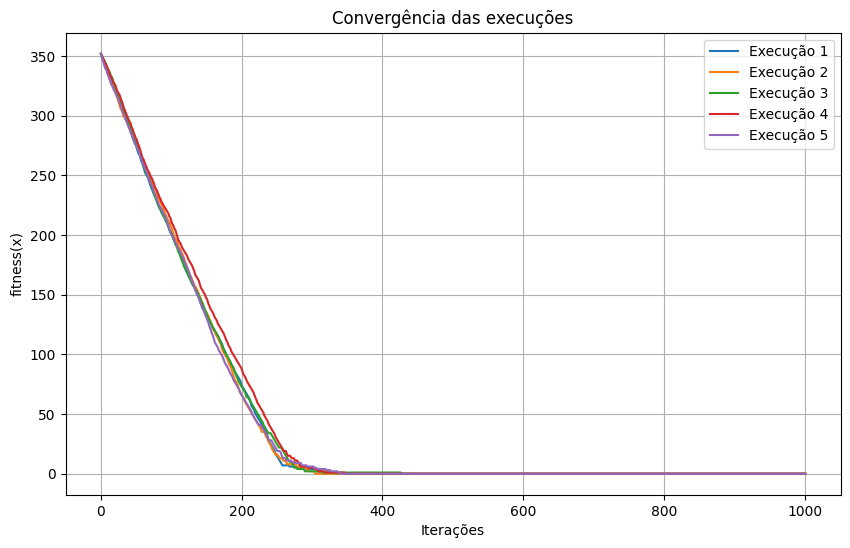
\includegraphics[width=\textwidth,trim=1 1 1 1,clip]{convergencia_execucoes_p1.png}
	\end{center}
	\legend{Fonte: elaboração própria.}
\end{figure}

Vemos que o algoritmo converge após 300 iterações para a solução 
ótima global, que já sabemos a priori uma vez que o problema modelado 
tem solução trivial. Cada iteração gastou em média 5 segundos para executar.

\section{Problema 2}

A \autoref{fig:convergencia_execucoes} mostra a convergência de 5 execuções
para o Problema 2. A solução final encontrada foi 

\[  \mathbf{x^*} = \begin{bmatrix} 2 & 2 & 2 & \cdots & 2 \end{bmatrix} \quad , \quad f\left(\mathbf{x^*}\right) = 1048.2 \pm 0 \]

\begin{figure}[h!]
	\caption{\label{fig:convergencia_execucoes}Convergência do BVNS implementado para o Problema 1 Isolado.}
	\begin{center}
    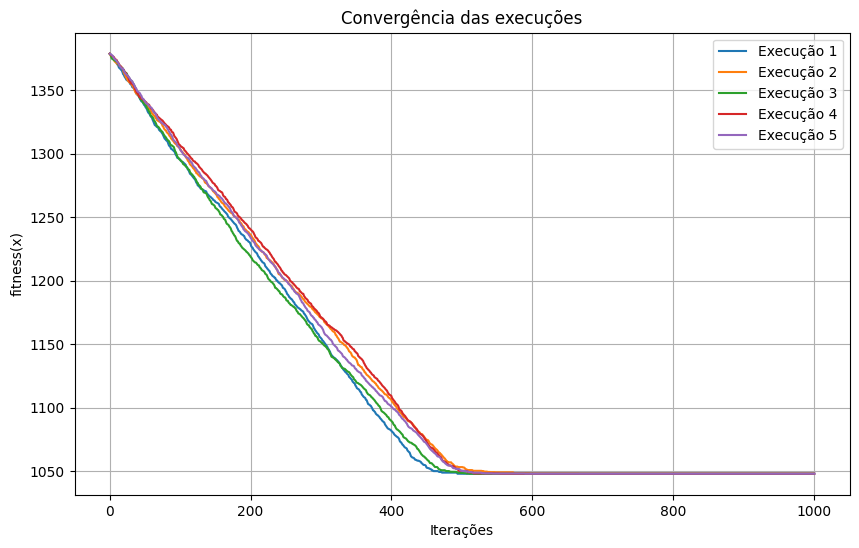
\includegraphics[width=\textwidth,trim=1 1 1 1,clip]{convergencia_execucoes.png}
	\end{center}
	\legend{Fonte: elaboração própria.}
\end{figure}

De forma similiar ao Problema 2, vemos que o algoritmo converge após 500 iterações para a solução 
ótima global dada pelo Simplex. Cada iteração gastou em média 12 segundos para executar.

\section{Comparação de Estratégias de Refinamento}

As convergências das Figuras \ref{fig:convergencia_execucoes_p1} e \ref{fig:convergencia_execucoes}
foram obtidas usando o BVNS com o FirstImprovement. Com o BestImprovement, obtemos 
as convergências das Figuras \ref{fig:bestImprovement_p1} e \ref{fig:bestImprovement_p2} para os Problemas 1 e 2, 
respectivamente.

\begin{figure}[h!]
	\caption{\label{fig:bestImprovement_p1}Convergência do BVNS implementado para o Problema 1 usando a Best Improvement.}
	\begin{center}
    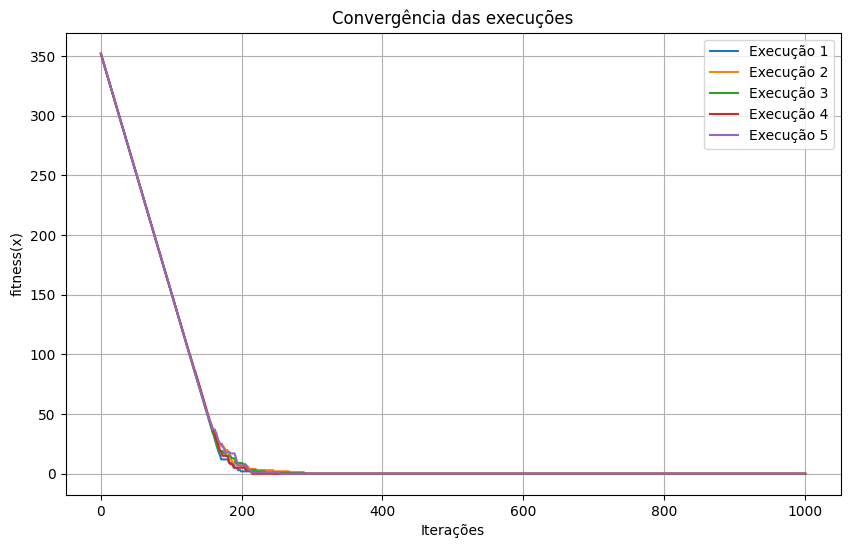
\includegraphics[width=\textwidth,trim=1 1 1 1,clip]{bestImprovement_p1.png}
	\end{center}
	\legend{Fonte: elaboração própria.}
\end{figure}

\begin{figure}[h!]
	\caption{\label{fig:bestImprovement_p2}Convergência do BVNS implementado para o Problema 2 usando a Best Improvement.}
	\begin{center}
    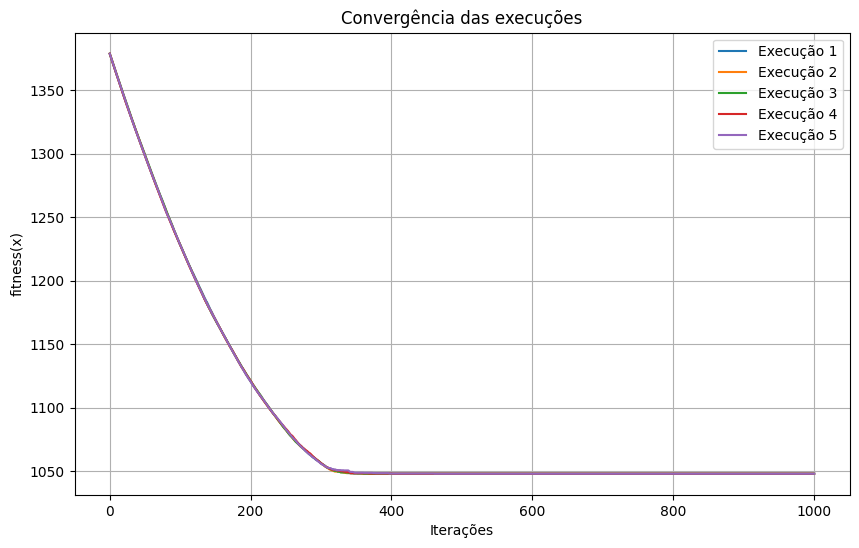
\includegraphics[width=\textwidth,trim=1 1 1 1,clip]{bestImprovement_p2.png}
	\end{center}
	\legend{Fonte: elaboração própria.}
\end{figure}

Vemos que com o BestImprovement o algoritmo converge com menos iterações quando comparado com o FirstImprovement:
antes precisava de 300 e 500 iterações respectivamente; agora converge em 200 e 300.
Contudo,
ele gasta mais tempo para executar uma vez que o custo computacional de cada iteração é maior.
Em particular, o Problema 2 gasta mais de 40 segundos por execução com o Best Improvement, sendo que antes gastava
apenas 12.
Não obstante, ambas estratégias convergiram para a mesma solução ótima global.

% \section{Comparação de Heurísticas Construtivas}

% Por fim, podemos comparar a convergência para o Problema 2, usando a FirstImprovement, entre execuções
% que usam ou não a heurística construtiva do Algoritmo \ref{alg:sol-inicial}. A \autoref{fig:semConstrutiva_p2} mostra 
% a convergência sem usar a heurística construtiva, isto é, usando uma solução inicial aleatória.

% \begin{figure}[h!]
% 	\caption{\label{fig:semConstrutiva_p2}Convergência do BVNS para o Problema 2 sem usar a heusrística construtiva.}
% 	\begin{center}
%     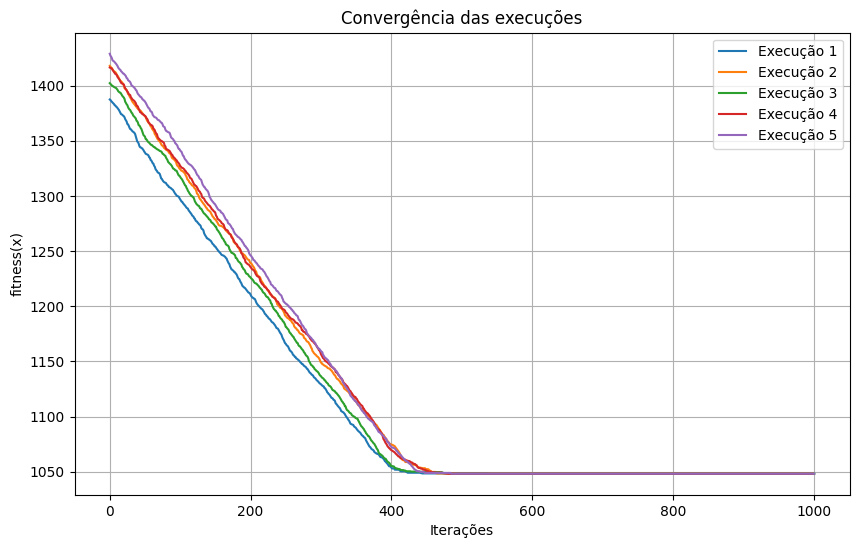
\includegraphics[width=\textwidth,trim=1 1 1 1,clip]{semConstrutiva_p2.png}
% 	\end{center}
% 	\legend{Fonte: elaboração própria.}
% \end{figure}

% Comparando as Figuras \ref{fig:semConstrutiva_p2} e \ref{fig:convergencia_execucoes}, vemos que a heurística construtiva 
% adotada consegue convergir mais rapidamente que algumas solução iniciais aleatórias. No entanto, ainda temos soluções aleatórias 
% que convergem mais rápido, indicando que é possível pensar em uma solução inicial melhor para o problema.

\chapter{Referências}\label{cap:referencias} 

\noindent M. Gendreau, J.-Y. Potvin (eds.), Handbook of Metaheuristics, Springer, 2nd ed., 2010.

\end{document}
